\chapter{Introduction to virtualization}



\section{What is virtualization?}

Today, virtualization is a broad term that refers to the abstraction computer
resources. It has been widely used since the 1960s or earlier, and has been
applied to many different aspects and scopes of computing — from entire
computer systems to individual capabilities or components. The common theme of
all virtualization technologies is the hiding of technical detail.

\begin{quote}
Virtualization is, at its foundation, a technique for hiding the physical
characteristics of computing resources from the way in which other systems,
applications, or end users interact with those resources. This includes making
a single physical resource (such as a server, an operating system, an
application, or storage device) appear to function as multiple logical
resources; or it can include making multiple physical resources (such as
storage devices or servers) appear as a single logical resource.~\cite{ema101}
\end{quote}

\begin{center}
\rule{10.0em}{0.02em}
\end{center}

\begin{quote}
Virtualization is a framework or methodology of dividing the resources of a
computer into multiple execution environments, by applying one or more concepts
or technologies such as hardware and software partitioning, time-sharing,
partial or complete machine simulation, emulation, quality of service, and many
others.~\cite{singh-intro}
\end{quote}

\begin{center}
\rule{10.0em}{0.02em}
\end{center}

\begin{quote}
Virtualization is an abstraction layer that decouples the physical hardware
from the operating system to deliver greater IT resource utilization and
flexibility.

Virtualization allows multiple virtual machines, with heterogeneous operating
systems to run in isolation, side-by-side on the same physical machine. Each
virtual machine has its own set of virtual hardware (e.g., RAM, CPU, NIC, etc.)
upon which an operating system and applications are loaded. The operating
system sees a consistent, normalized set of hardware regardless of the actual
physical hardware components.~\cite{vmware-intro}
\end{quote}

Due to the abstract nature of these definitions the list of virtualization
types, implementations and frameworks is rather huge, and we trust that readers
will appreciate that this subject cannot be covered in great detail here.
Nevertheless the following list encompasses some popular virtualization
techniques, to give the reader -- at least -- a rough understanding of key
differences between current major technologies.

A rather complete list of virtualization frameworks can be found on Amit Singhs
page \textit{An Introduction to Virtualization}.~\cite{singh-intro}


\section{Simulation}

A \textit{computer simulation} is an attempt to model a real-life situation on
a computer so that it can be studied to see how the system works. By changing
variables, predictions may be made about the behaviour of the system.

An interesting application of computer simulation is to simulate computers
using computers. The related software is called computer architecture
simulators, which can be further divided into instruction set simulators or
full system simulators.

An instruction set simulator is often provided with a debugger in order for a
software engineer to debug the program prior to obtaining target hardware.  GDB
is one of debuggers which have compiled-in ISS. It is sometimes integrated with
simulated peripheral circuits such as timers, interrupts, serial port, general
I/O port, etc to mimic the behavior of microcontroller.~\cite{wp-iss}


\section{Emulation}

A \textit{Software Emulator} allows computer programs to run on a platform
(computer architecture and/or operating system) other than the one for which
they were originally written. More generally, emulation refers to the ability
of a program or device to imitate another program or device.

Many printers, for example, are designed to emulate Hewlett-Packard LaserJet
printers because so much software is written for HP printers. By emulating an
HP printer, a printer can work with any software written for a real HP printer.
Emulation tricks the software into believing that a device is really some other
device.

Another  popular use of emulators is to mimic the experience of running arcade
games or console games on personal computers. Emulating these on modern desktop
computers is usually less cumbersome and more reliable than relying on the
original machines, which are often old and hard to find, let alone repair.
Emulation of arcade and console systems on home PCs usually includes the
practice of illegally downloading software from various electronic distribution
sources.

In a theoretical sense, the Church-Turing thesis~\cite{church-turing}
implies that any operating environment can be emulated within any other. In
practice, however, it can be quite difficult, particularly when the exact
behavior of the system to be emulated is not documented and has to be deduced
through reverse engineering. It also says nothing about timing constraints --
if the emulator does not perform as quickly as the original hardware, the
emulated software may run much more slowly than it would have on the original
hardware.


\section{Simulation vs. Emulation}

There is a lot of confusion between emulators and simulators, in fact, the
distinction between those two is not always easy to tell. Ed
Thelen~\cite{emu-vs-simu} has collected some opinions on the difference, some of
which are quoted below.

In October 2005, Peter Hans van den Muijzenberg wrote:

\begin{verbatim}
Hi,

Regarding the difference between simulation and emulation:
Not limited to computers I use this distinction:
- A simulation mimics the outward appearance
- An emulation mimics the cause/process.

If you want to convince people that watching television gives you
stomach-aches, you can simulate this by holding your chest/abdomen and
moan. You can emulate it by eating a kilo of unripe apples.

BFN,
                                Peter Hans van den Muijzenberg
\end{verbatim}

Another, quite theoretical view of the problem, from Arun Parajuli, January
2006:

\begin{verbatim}
In my view the difference between simulation and emulation is:

Emulation: A system X is said to emulate another system Y if the
behaviour of X is exactly the same as that of Y (same out put for
same input under similar conditions) but the mechanism to arrive at
the output (from the input) is different.  Emulation is generally
used when we don't exactly know the internal mechanism of the
original system but are familiar with the input/output pattern. For
example, neural networks may be used to emulate different systems.
Neural networks are trained to produce the same output for the same
input as that of the original system though the mechanism/procedure
to generate the output are quite different.

Simulation: A system X is said to simulate another system Y
when the internal mechanism/procedures of X is a mathematical
(or any other) model known to best represent the actual mechanism
of Y. Simulation is generally used when we have some mathematical
models of the original system (Y) and want to know output for a
given set of inputs. For example we may have a good mathematical
model of effect of water temperature on the hurricane formation. We
use that system to predict the nature of hurricanes for different
water temperatures. It is to be noted that the result of simulation
can sometimes be unverifiable. For example the hurricane pattern
suggested by the simulator for water temperature equal to 50 degree
Celsius will be difficult to verify because we may never encounter
such situation.

Arun Parajuli
\end{verbatim}


\section{Native Virtualization}

Native virtualization, in which the Virtual Machine simulates complete hardware
to allow operation of an umodified operating system for the same type of CPU to
execute within the virtual machine container in complete isolation.

\begin{figure}[H]
	\center
	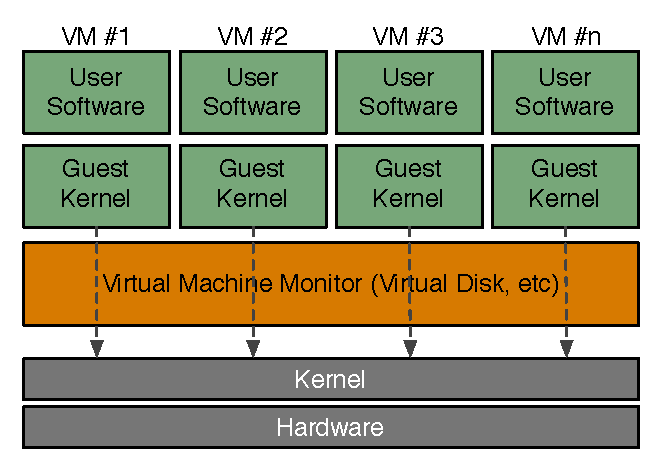
\includegraphics[scale=0.75]{intro/native-virtualization}
	\caption{Native Virtualization}
\end{figure}

Native virtualization leverages hardware-assisted capabilities available in the
latest processors from Intel (Intel VT) and Advanced Micro Devices (AMD-V) to
provide near-native performance. Prior to these processors, the x86
architecture did not meet some fundamental requirements for virtualization,
making it difficult to implement a virtual machine monitor for this type of
processor.

These requirements include: equivalence - a program running under the virtual
machine should exhibit a behavior essentially identical to the original
physical machine; resource control - the virtual machine must be in complete
control of the virtualized resources and efficiency - where the virtual machine
should not significantly degrade workload performance.~\cite{wp-native-virt}

\section{Para-virtualization}

However, native virtualization may incur a performance penalty.  The VM monitor
must provide the VM with an image of an entire system, including virtual BIOS,
virtual memory space, and virtual devices. The VM monitor also must create and
maintain data structures for the virtual components, such as a shadow memory
page table. These data structures must be updated for every corresponding
access by the VMs.

\begin{figure}[H]
	\center
	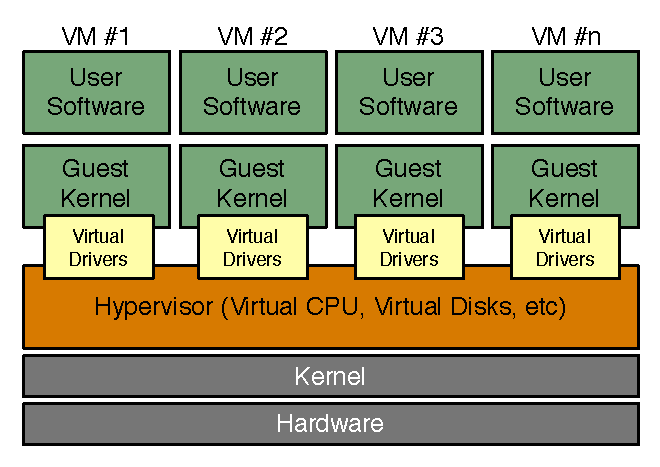
\includegraphics[scale=0.75]{intro/para-virtualization}
	\caption{Para-Virtualization}
\end{figure}

Therefore, para-virtualization exposes a virtual architecture that is slightly
different than the physical architecture. The differences in the architecture
are driven by improvements in scalability or reductions in system complexity.
Modifying the architecture breaks backwards compatibility with existing OS
code, which is a major disadvantage. However, it enables to co-design the
virtual architecture with the operating system, which gives a considerable
latitude when exploring issues of scale.

Para-virtualization has been used in previous VMMs, including VM/370 and Disco.
These systems added a combination of instructions, registers, or devices to the
virtual architecture to improve performance. However, because the goal of these
systems was to run legacy OSs, their use of para-virtualization was
minimized.~\cite{denali}

Porting an operating system to run on the VMM is similar to supporting a new
hardware platform, however the process is simplified because the para-virtual
machine architecture is very similar to the underlying native hardware.

The term ``para-virtualization'' was first used in the research literature in
association with the Denali virtual machine monitor~\cite{denali}. The term
is also used to describe the Xen, L4, Virtual, Iron and TRANGO hypervisors. All
these projects use paravirtualization techniques to support high performance
virtual machines on x86 hardware.


\section{Operating System-Level Virtualization}

\textit{Operating System-Level Virtualization} is a server virtualization
technology which virtualizes servers on a operating system (kernel) layer. It
can be thought of as partitioning a single physical server into multiple small
computational partitions. Each such partition looks and feels like a real
server, from the point of view of its owner. On Unix systems, this technology
can be thought of as an advanced extension of the standard chroot mechanism.

\begin{figure}[H]
	\center
	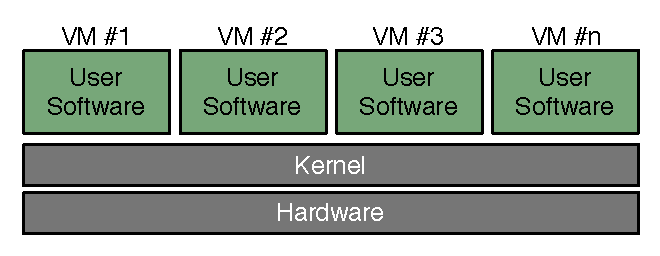
\includegraphics[scale=0.75]{intro/os-virtualization}
	\caption{Operating System-Level Virtualization}
\end{figure}

Many terms for the computational partitions exist and mostly depend on the
implementation: virtual environments (VE), virtual private servers (VPS),
jails, guests, zones, vservers, containers, etc.

The operating system level architecture has low overhead that helps to maximize
efficient use of server resources. Due to a single-kernel approach, this type
of virtualization introduces only a negligible overhead and allows running
hundreds of virtual private servers on a single physical server. In contrast,
approaches such as emulation and para-virtualization cannot achieve such level
of density, due to overhead of running multiple kernels. On the other hand,
operating system-level virtualization does not allow running different
operating systems (i.e. different kernels), although different libraries,
distributions etc. are possible.~\cite{wp-os-virt}
